\documentclass{article}
\usepackage{ragged2e} 
\usepackage{amsmath} 
\usepackage{amsmath}
\usepackage{hyperref}
\usepackage[T1]{fontenc}
\usepackage[utf8]{inputenc}
\usepackage[english]{babel} 
\usepackage{graphicx}
\graphicspath{ {./imgs/} }
\usepackage{float}
\usepackage{listings}
\usepackage{xcolor}
\usepackage{url}

\urlstyle{rm}
\sloppy

\title{Simulation of the impact of changes in the capital structure of an enterprise on its market value using neural networks}
\author{Monika Etrych, Kacper Sobczyk}
\date{March 2024}

\begin{document}

\maketitle
\centering etrych@student.agh.edu.pl ksobczyk@student.agh.edu.pl
\begin{flushleft}
\begin{justify}

\section{Introduction}
\subsection{Theoretical Introduction}
\subsubsection{Structural Capital}
The aim of this project is to implement and train neural network based on
economic dataset. We are going to predict market value based on impact of
changes in the capital structure of an enterprise.

The capital structure of a company has been a central topic in modern fi-
nance theory for over four decades. It has not only gained formal recognition
in recent years but also continues to attract the attention of researchers, high-
lighting its significance. [1] Capital, being one of the fundamental economic
categories, is at the same time a multifaceted concept subject to various in-
terpretations. It is this complexity and versatility that make the analysis of a
company’s capital structure crucial for understanding the financial dynamics of
the market and for the strategies of corporate financial management. [2]
Capital, when considered at an abstract level, is seen as an economic value
with the potential for growth. This increase in value leads to the creation of
what is known as ’added value’, understood as profit or interest. Possessing
capital turns out to be an essential condition not only for establishing but also
for the functioning and development of every economic entity. In a more tangible
dimension, capital is captured as financial resources or tangible goods used in
the production process, aimed at stimulating further development of production.
[3]

The conscious shaping and assessment of a company’s capital structure,
which is the analysis of the relationships and proportions between different types of financial resources, becomes a key task for managers. The concept of capital
structure primarily refers to the way in which a company’s sources of financing
are configured, including equity and debt, the cost of which is interest-bearing.
How a company manages its capital structure has a direct impact on its ability
to generate added value, as well as on its financial stability and developmental
possibilities in the long term. In the context of these considerations, a thorough
understanding and effective management of the capital structure emerge as key
challenges for any company striving for success in the market. [4]

Equity capital plays a pivotal role in the functioning of a company, enabling
not only the commencement of business operations but also providing financial
protection in the event of incurred losses or the need to repay funds borrowed
from creditors. Simultaneously, it serves as a source of financing for current
business operations. In theory, funding a company exclusively through equity
is considered the safest option, which minimizes financial risk. However, in
practice, raising equity capital is associated with higher costs compared to debt
capital, and it also limits the ability to utilize the financial leverage effect.
On the other hand, debt capital primarily arises from obligations to creditors
and is characterized by lower acquisition costs. It allows for the implementation
of certain tax optimization strategies, but at the same time, it increases financial
risk and can negatively affect the perception of the company’s creditworthiness.
Thus, while debt capital offers a range of benefits, including cost advantages,
it also comes with an increased level of risk, which requires prudent financial
management of the company. [5]

\subsubsection{1.1.2 Determinants of the Capital Structure of the Enterprise}

The determinants of the capital structure of an enterprise are complex and
multifaceted, encompassing both internal factors related to the activity and
characteristics of the firm itself, and external factors resulting from the macroe-
conomic environment. Here is a summary of the factors determining the capital
structure of the enterprise, divided into internal (microeconomic) and external
(macroeconomic). [6]

Microeconomic factors:
\begin{itemize}
\item{Company size}
\item{The industry in which the company operates}
\item{Cost of capital}
\item{Financial liquidity}
\item{Level of risk acceptance}
\item{Perception of the company’s own market position}
\item{The size of assets in the company (asset structure)}
\item{Profitability of the company}
\item{Dividend policy in the company}
\item{Adopted investment strategy}
\end{itemize}

Macroeconomic factors:
\begin{itemize}
\item{The level of economic development of the country (the level of inflation
and interest rates)}
\item{Fiscal policy conducted}
\item{Legal regulations}
\item{The size and efficiency of the banking sector}
\item{The level of technological advancement available in the country}
\item{The level of development of financial markets (including the development
of emerging markets and their impact on the debt capacity of large enter-
prises)}
\end{itemize}

Both microeconomic and macroeconomic factors not only influence the choice
of the capital structure of the enterprise but also have significant importance
in shaping its value. Through conscious analysis and adaptation to these de-
terminants, enterprises can not only optimize their financial decisions but also
increase their value in the market.


\subsubsection{Market Value of the Enterprise and the Impact of Structural Capital}

The market value of an enterprise reflects the price at which it can be purchased
or sold under conditions of an open and competitive market, assuming that the
transaction is conducted fairly and that both parties act rationally, having an ad-
equate amount of information. This definition, proposed by Wójcik-Jurkiewicz
in 2009, emphasizes the importance of transparency and access to information
for determining the fair market value of an enterprise. [7]

In the discussion on methods of assessing the value of an enterprise, prac-
titioners and financial theorists agree on the importance of various financial
indicators. [8] Rappaport highlights both classic indicators such as return on
equity, sales growth, investments in fixed assets, or changes in working capital,
as well as those that go beyond the direct financial ties of the enterprise, such
as competitive advantages. [9] Contemporary economic approaches, represented
among others by Damodaran in 2017, point to the maximization of enterprise
value as the primary goal of business activity. [10] For public companies, whose
shares are listed on the stock exchange, this goal takes on a particularly mea-
surable character - maximizing market value means striving to raise the price
of shares, which directly translates into the satisfaction of shareholders. [8]

Understanding the market value of an enterprise can vary, however, in the
stock market context, it is often equated with market capitalization, that is, the stock market value of the company, defined as the product of the number of shares in circulation and their current market price. This perspective allows
for a clear determination of the company’s value in the financial market, which
is especially important for investors and shareholders analyzing the investment
potential of the company. The market value of the enterprise is expressed as the
product of the price of one share and the total number of shares of the enterprise
in circulation, which can be represented by the equation:

\begin{equation} W_{p} = k_{a} \cdot l_{A} \end{equation}
where:
\[ W_{p} \text{ - market value of company} \]
\[ k_{a} \text{ - share price} \]
\[ l_{A} \text{ - number of total shares of the company} \]


\subsection{Review of Current Research}
\subsubsection{Solutions Used in Economics and Finance}

Over the past decades, the dynamic development of information technology has
significantly impacted the financial sector, opening up new possibilities for data
analysis and optimization of investment strategies. [11] A key aspect of this
transformation is the implementation of machine learning (ML) and deep learn-
ing (DL) algorithms in financial processes, revolutionizing the way data is pro-
cessed and interpreted. [12] Machine learning algorithms, both supervised and
unsupervised, rely on mathematical data modeling, with the main goal being to
minimize errors and increase the predictive accuracy of the model. Traditional
methods, such as support vector machines (SVM), decision trees, and random
forests, have found widespread application in finance - from regression analy-
sis to real estate price forecasting, credit card fraud detection, to stock price
movement prediction. [13]

In recent years, deep learning has garnered special interest, building on the
foundation of machine learning. Such architecture allows for the processing of
complex financial problems, providing tools capable of analyzing and interpret-
ing data at a level unreachable by traditional methods. The use of AI and ML
in finance opens up new possibilities for market forecasting, investment strategy
optimization, and risk management, while also providing greater accuracy and
speed in making key business decisions. Neural networks are advanced mathematical algorithms designed after the
human brain. They are inspired by biological neural networks, where individual
neurons transmit signals via synapses. Similarly, in artificial neural networks,
information moves between nodes (corresponding to neurons) through connec-
tions, whose strength, or weights, can be adjusted during the learning process.
[13]

This analogy to the human brain not only gives neural networks the ability
to solve complex problems through learning and adaptation but also allows for
the processing and interpretation of data in a way more akin to human thinking
and perception. Through iterative adjustment of weights based on training data,
neural networks can ”learn” to recognize patterns, predict outcomes, and make
decisions with remarkable accuracy. [13]

In practice, this means that neural networks are capable of learning and
evolving, adjusting their weights based on input data, which allows them to
identify patterns and trends that may not be visible to the human eye or through
traditional analysis methods. Thanks to this ability to learn and adapt, neu-
ral networks find wide application in various fields, such as image recognition,
natural language processing, financial forecasting, and many more.

\subsubsection{Examples of Neural Network Architectures}


\begin{align*}
& \text{MLP} & - & \text{Multilayer Perceptron} \\
& \text{RNN} & - & \text{Recurrent Neural Network} \\
& \text{LSTM} & - & \text{Long Short Term Memory} \\
& \text{CNN} & - & \text{Convolutional Neural Network}
\end{align*}


\subsection{Citations}
[1] The Dynamics of Capital Structure, Saugata Banerjee, Almas Heshmati, Clas
Wihlborg url: \url{https://citeseerx.ist.psu.edu/document?repid=rep1&type=
pdf&doi=d96373c220255e4d055d172f0ad7df58834982dc} (str.1)

[2] Determinanty struktury kapitalu w przedsiebiorstwie* - Sylwia Betkowska**
(str. 386)

[3] Determinanty struktury kapitalu w przedsiebiorstwie* - Sylwia Betkowska**
(Borowiecki, Czaja, Jaki 1998, s. 21 – cytowanie wt´orne str 387.).

[4] 3. A. Cwynar, W. Cwynar, Optymalizacja struktury kapitalu i kalkulacja
kosztu kapitalu spółki, w: Finansowanie rozwoju przedsiebiorstwa, red. M.
Panfil, Difin, Warszawa 2008, s. 57.

[5] A. Kwiecień. Struktura kapitalu a stopa zwrotu – analiza przypadku”.
Polish. W: Studia Ekonomiczne 222 (2015), s. 139–152.

[6] DETERMINANTY STRUKTURY KAPITALOWEJ PRZEDSIEBIORSTWA1
– Agnieszka Kurczewska str, 327, 329 Uniwersytet L´odzki url: \url{https://dbc.wroc.pl/Content/121395/Kurczewska_Determinanty_struktury_kapitalowej.pdf}

[7] MODEL SZACOWANIA WARTOŚCI PRZEDSIĘBIORSTWA NA POD-
STAWIE DANYCH PUBLIKOWANYCH PRZEZ GIELDE PAPIERÓW WARTO-ŚCIOWYCH
W WARSZAWIE Sara RUPACZ1 , Izabela JONEK-KOWALSKA 2*, str. 111-
113 url: \url{https://zij.edu.pl/wp-content/uploads/2022/09/Vol-4-No-3-NOWY_merged-110-130.pdf}

[8] ROLA PRZEDSIEBIORCY W BUDOWANIU WARTOŚCI PRZEDSIEBIORSTWA
RODZINNEGO. Str 135, Adriana Kaszuba-Perz, Pawel Perz

[9] Rappaport A. (1999), Warto´s´c dla akcjonariuszy, Wig-Press, Warszawa.

[10] Damodaran A. (2017), Finanse korporacyjne. Teoria i praktyka, Onepress, Gliwice

[11] AI-Based Prediction of Capital Structure: Performance Comparison of ANN
SVM and LR Models Jesus Cuauhtemoc Tellez Gaytan, 1 Karamath Ateeq, 2 Aqila Rafiuddin, 3 Haitham M. Alzoubi, 4 Taher M. Ghazal, 2,5 Tariq Ahamed Ahanger, 6 Sunita Chaudhary, 7 and G. K. Viju 8

[12] Stock Prediction Using Convolutional Neural Network Sheng Chen1, * and
Hongxiang He \url{https://iopscience.iop.org/article/10.1088/1757-899X/435/1/012026/pdf}

[13] An introduction to neural networks Kevin Gurney University of Sheffield, pages 3-6

[14] Medium, "Understanding Recurrent Neural Network (RNN) and Long Short Term Memory(LSTM)" -Vijay Choubey, \url{https://medium.com/analytics-vidhya/undestanding-recurrent-neural-network-rnn-and-long-short-term-memory-lstm-30bc1221e80d}



\section{Problem formulation and proposed solution}
\subsection{Problem formulation}
opis rozwiązywanego problemu...
to do
\subsection{Algorithms}
\subsubsection{RNN - Recurrent Neural Networks}
RNN is a type of neural network which contains memory about previous data and it is best suited for sequential data. RNN remembers old data to help it make decisions based on what it's currently seeing. 

In each iteration of the process, the input data is multiplied by a set of weights . Subsequently, new input data is introduced along with the output data from the previous iteration, which is also multiplied by these weights. [14]

\begin{figure}[H]
\centering 
\caption{Recurrent Neural Network}
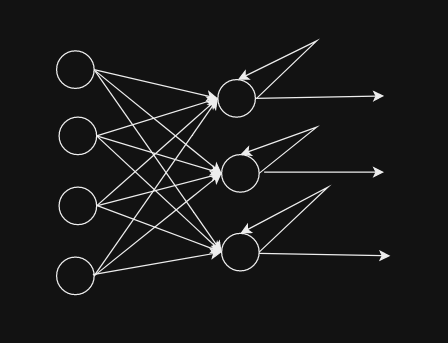
\includegraphics{imgs/rnn.png}

\small Image source: Created by the author 
\end{figure}




\begin{figure}[H]
\centering 
\caption{Types of Recurent Neural Networks}
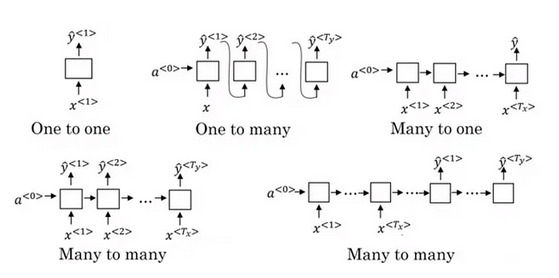
\includegraphics{imgs/rnn_types.PNG}
\small Image source: \url{https://medium.com/analytics-vidhya/undestanding-recurrent-neural-network-rnn-and-long-short-term-memory-lstm-30bc1221e80d}
\end{figure}

\textbf{There are four types of RNNs:}

- One to One:

- One to Many

- Many to One:

- Many to Many

\vspace{1em}

The types divides networks by amount of inputs and outputs. The most basic type is One to One, it is also called Vanilla. It has only one layer with only one input and output. One to Many contains many layers with one input and many outputs. The following types works similarly.

In this problem we will use Many to One RNN because we provide many time series as input and we will get one company market value as output.

\vspace{1em}

\textbf{RNNs has two main problems:}

- \textbf{Vanishing Gradient} - gradient values are too small. In this situation model learns incredibly slow or even stops learning.

-\textbf{ Exploding Gradient} - gradient values are too big. In this case, learning is highly unstable, loss function instead of decreasing it is increasing extremely fast. Exploding gradients are typically a result of issues related to network architecture .

Due to vanishing gradient, RNN does not have ability to capture long-term dependencies in sequential data. This capability makes LSTMs better suited for tasks requiring the modeling of complex sequential patterns and dependencies compared to traditional RNNs. So it is why we have decided to use this cell[14].

\subsubsection{LSTM - Long Short Time Memory}

LSTM in comparison to RNN can decide if information can be useful in the future or not. The gates are responsible for classifying information for important and not. These three gates are:

- input gate

- output gate

- forget gate
\vspace{1em}
\textbf{Forget gate:} This gate decide which information is important and should be stored and which information to forget. It counts 'validity coefficient' and  assigns every information a value in range 0 to 1. Near 0 means that information is non important and near 1 means that information is important. This value is counted based on output data from previous layer and input data from current layer and all other coefficients. It is like one step in recurrent network.

\textbf{Input Gate:} Generates values in range -1 to 1 which should be added function operating one step in recurrent neural network.

\textbf{Output Gate:}  This gate is responsible for selecting important information from current cell and show it as output.

\vspace{1em}

In our project we will use Tensorflow to create recurrent neural network with LSTM cell. In base model we have added 1 LSTM cell and one Dense output layer with one neuron. We realize that it can be too small network but it is our first one from which we will start.

\lstdefinestyle{mystyle}{
    commentstyle=\color{codegreen},
    keywordstyle=\color{blue},
    basicstyle=\footnotesize\ttfamily
}

\lstset{
    language=Python,
    basicstyle=\small\ttfamily,
    keywordstyle=\color{blue},
    showstringspaces=false,
    breaklines=true, 
    frame=single,
    numbers=left,
    numberstyle=\tiny,
    captionpos=b
}

\lstset{style=mystyle, morekeywords={Sequential, LSTM, Dense}}

\begin{lstlisting}[caption={Example Python code}, label=lst:example]
model = Sequential()
model.add(LSTM(50, input_shape=(train_X.shape[1], train_X.shape[2])))
model.add(Dense(1))
model.compile(loss='mae', optimizer='adam')
\end{lstlisting}






\subsection{Libraries}
To create this project we have used python 3.10 and the following libraries:

•	scikit-learn (sklearn): Machine learning library offering tools for data preprocessing, model building, and evaluation.

•	Pandas: Data manipulation and analysis library, perfect for data tables.

•	TensorFlow: Deep learning library for building and training neural networks.

•	Matplotlib: Plotting library for creating visualizations like charts and graphs.



\section{Experimental research results}



\section{Summary and conclusions}

\end{justify}
\end{flushleft}
\end{document}
